\documentclass{beamer}
\usetheme{metropolis}
\usepackage{graphicx}
\usepackage{caption}
\usepackage{amsmath}
\usepackage{hyperref}
\usepackage{tikz}
\usetikzlibrary{circuits.ee.IEC,positioning}
\usepackage{pgfplots}
\pgfplotsset{compat=1.18}
\title{Reliability Engineering 101 for NSWC Corona}
\author{Jordan Hanson}
\institute{Whittier College Department of Physics and Astronomy}
\definecolor{mBlack}{RGB}{0,0,0}
\definecolor{mGray}{RGB}{64,64,64}
\setbeamercolor{normal text}{fg=mBlack}
\setbeamercolor{alerted text}{fg=mGray}
\captionsetup[table]{font=scriptsize}
\captionsetup[figure]{font=scriptsize}

\begin{document}
\maketitle

\begin{frame}{Outline}
\small
\textbf{Part I : Introduction and Mathematics}
\begin{itemize}
\item 1.1 : Scope of Reliability Engineering
\begin{itemize}
\item 1.1.1 : NAVSEA Documentation on Reliability
\item 1.1.2 : Impact of Reliability
\item 1.1.3 : Knowing our Systems
\item 1.1.4 : Model and Method Selection
\item 1.1.5 : Model Development
\end{itemize}
\item 1.2 : Mathematics of Reliability Engineering
\begin{itemize}
\item 1.2.1 : Statistics and Probability
\item 1.2.2 : Probability Distribution Functions (PDFs)
\item 1.2.3 : Estimation and Hypotheses Testing
\item 1.2.4 : Graphical and Tabular Methods
\item 1.2.5 : Goodness-of-Fit Tests
\item 1.2.6 : Regression Analysis
\end{itemize}
\end{itemize}\end{frame}
\begin{frame}{Outline}
\small
\textbf{Part II : Reliability of Components and Systems}
\begin{itemize}
\item 2.1 : Reliability of Components
\begin{itemize}
\item 2.1.1 : Reliability Functions : $f(t)$, $F(t)$, $R(t)$, and $h(t)$
\item 2.1.2 : Common PDFs for Reliability Functions
\item 2.1.3 : Model Selection and Parameter Estimation
\begin{itemize}
\item Application of Maximum-Likelihood Estimators (MLEs)
\item Non-parametric Estimators
\item Bayesian Techniques
\end{itemize}
\end{itemize}
\item 2.2 : Reliability of Systems
\begin{itemize}
\item 2.2.1 : Reliability Block Diagrams (RBDs)
\item 2.2.2 : Success and Fault Tree Analysis
\item 2.2.3 : Failure Mode and Effect Analysis (FMEA/FMECA)
\end{itemize}
\end{itemize}
\end{frame}
\begin{frame}{Outline}
\small
\textbf{Part III : Reliability and Availability of Repairable Systems}
\begin{itemize}
\item 3.1 : Reliability of Repairable Systems
\begin{itemize}
\item 3.1.1 : Point Process Definition and Homogeneous Point Processes (HPPs)
\item 3.1.2 : Non-Homogeneous Point Processes (NHPPs) and Renewal Processes
\item 3.1.3 : Analysis Techniques for HPPs and NHPPs
\item 3.1.4 : Availability of Repairable Systems
\item 3.1.5 : Availability of Complex Systems
\end{itemize}
\item 3.2 : Selected Topics in Reliability Data Analysis
\begin{itemize}
\item 3.2.1 : System Classification (One-shot, repairable)
\item 3.2.2 : Reliability Data, Type and Classification
\end{itemize}
\end{itemize}
\end{frame}

\section{Part I: Introduction and Mathematics}

\begin{frame}{Module 1.2.3 : Estimation and Hypothesis Testing}
\begin{columns}[T]
\begin{column}{0.52\textwidth}
\small
\textbf{Point estimation} uses sample data to estimate
unknown parameters of a probability distribution.
\begin{itemize}
\small
\item Population parameters
\begin{itemize}
\scriptsize
\item Mean ($\mu$)
\item Standard deviation ($\sigma$)
\item Failure rate ($\lambda$)
\item Weibull parameters ($\beta,\eta$)
\end{itemize}
\item Sample estimates
\begin{itemize}
\scriptsize
\item Sample mean ($\bar{x}$)
\item Sample standard deviation ($s$)
\item Maximum likelihood estimators (MLEs)
\end{itemize}
\end{itemize}
\end{column}
\begin{column}{0.48\textwidth}
\begin{tikzpicture}
\begin{axis}[
width=\linewidth,
height=5cm,
xmin=-3,
xmax=3,
ymin=0,
ymax=0.45,
axis lines=left,
xlabel={$x$},
ylabel={$f(x)$},
xtick={0},
xticklabels={$\mu$},
ytick=\empty
]
\addplot[domain=-3:3,samples=200,thick,gray]{1/sqrt(2*pi)*exp(-x^2/2)};
\addplot[only marks,mark=*,mark size=2pt]
coordinates{
(-1.2,0.04)
(-0.8,0.10)
(-0.3,0.22)
(0.2,0.36)
(0.7,0.26)
(1.0,0.15)
};
\draw[dashed](axis cs:0.15,0)--(axis cs:0.15,0.39);
\node[above] at (axis cs:0.15,0.4){\scriptsize $\bar{x}$};
\end{axis}
\end{tikzpicture}
\scriptsize
\textbf{Sample mean : } Estimate the population mean from a finite sample.
\begin{equation}
\bar{x}=\frac{1}{n}\sum_{i=1}^n x_i
\end{equation}
Formulas for mean and variance are different for various PDFs.
\end{column}
\end{columns}
\end{frame}

\begin{frame}{Module 1.2.3 : Estimation and Hypothesis Testing}
\begin{columns}[T]
\begin{column}{0.52\textwidth}
\small
\textbf{Confidence intervals} quantify the uncertainty in an estimated parameter.
\begin{itemize}
\small
\item Point estimates are never exact.
\item Larger samples produce narrower intervals.
\item Confidence levels are commonly
\begin{itemize}
\small
\item 90\%
\item 95\%
\item 99\%
\end{itemize}
\end{itemize}
\end{column}
\begin{column}{0.48\textwidth}
\small
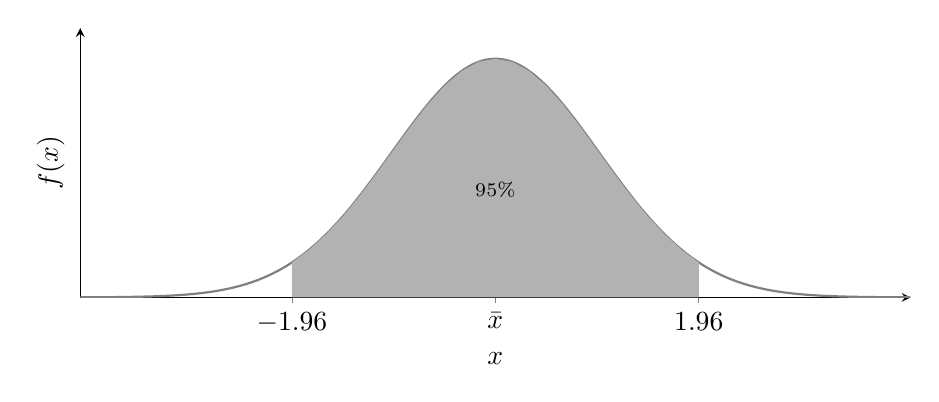
\begin{tikzpicture}
\begin{axis}[
width=\linewidth,
height=5cm,
xmin=-4,
xmax=4,
ymin=0,
ymax=0.45,
axis lines=left,
xlabel={$x$},
ylabel={$f(x)$},
xtick={-1.96,0,1.96},
xticklabels={$-1.96$,$\bar{x}$,$1.96$},
ytick=\empty
]
\addplot[domain=-4:4,samples=250,thick,gray]{1/sqrt(2*pi)*exp(-x^2/2)};
\addplot[domain=-1.96:1.96,draw=none,fill=black!30]{1/sqrt(2*pi)*exp(-x^2/2)}\closedcycle;
\node at (axis cs:0,0.18){\scriptsize 95\%};
\end{axis}
\end{tikzpicture} \\
The graph represents a 95\% confidence interval (CI) surrounding the estimated mean.  CI for confidence level $\alpha$:
\begin{equation}
\bar{x}\pm
z_{\alpha/2}\frac{\sigma}{\sqrt n}
\end{equation}
\end{column}
\end{columns}
\end{frame}

\begin{frame}{Module 1.2.3 : Estimation and Hypothesis Testing}
\begin{columns}[T]
\begin{column}{0.53\textwidth}
\scriptsize

\textbf{Example : } An electronic component is known to have an exponential failure distribution. A random sample of $n=12$ components is tested, producing a total operating time of $S=\sum_{i=1}^{12}t_i=8400$ hours. The estimated failure rate is

\begin{equation}
\hat{\lambda} = 1.43\times10^{-3} \text{hr}^{-1}.
\end{equation}

The estimate for $\hat{\lambda}$ is derived from the maximum likelihood estimator (MLE, next page).  Note that, for an exponential distribution, an exact CI for the failure rate is

\begin{equation}
\frac{\chi^2_{\alpha/2,\,2n}}{2S}<\lambda<\frac{\chi^2_{1-\alpha/2,\,2n}}{2S} \label{eq:lambda_mle}
\end{equation}
\end{column}

\begin{column}{0.47\textwidth}
\scriptsize
For a two-sided 95\% confidence interval ($\alpha = 0.05$, $n=12$), $\chi^2_{0.025,24}=12.40$, and $\chi^2_{0.975,24}=39.36$. \\ \vspace{0.25cm}

\textbf{Question : } (i) What is the 95\% CI for the failure rate, and (ii) what is the corresponding confidence interval for the MTTF, if $MTTF=\frac{1}{\lambda}$? \\ \vspace{0.25cm}

(i) Using Eq. \ref{eq:lambda_mle}, $7.38\times 10^{-4} \text{hr}^{-1} < \lambda < 2.34 \times 10^{-3} \text{hr}^{-1}$.  (ii) Take the lower bound for $\lambda$ as the inverse of the \textit{upper} bound for MTTF, and vice versa: $427\text{hr} < MTTF < 1355 \text{hr}$. \\ \vspace{0.25cm}

\textbf{How do we obtain} $\hat{\lambda}$?
\end{column}
\end{columns}
\end{frame}

\begin{frame}{Module 1.2.3 : Estimation and Hypothesis Testing}
\scriptsize
\textbf{Maximum Likelihood Estimation (MLE):}
Suppose $n$ independent failure times,
$t_1,t_2,\ldots,t_n$, are known to follow an exponential distribution
with failure rate $\lambda$. \\ \vspace{0.25cm}
\textbf{Question :}
How can the parameter $\lambda$ be estimated from the observed data?
\vspace{0.25cm}
\begin{columns}[T]
\begin{column}{0.58\textwidth}
\scriptsize
The likelihood function is
\begin{equation}
L(\lambda)=\prod_{i=1}^{n}\lambda e^{-\lambda t_i}=\lambda^n e^{-\lambda\sum t_i}.
\end{equation}
Taking the natural logarithm,
\begin{equation}
\ln L(\lambda)=n\ln\lambda-\lambda\sum t_i
\end{equation}
Differentiating and setting the result equal to zero,
\begin{equation}
\frac{d}{d\lambda}\ln L=\frac{n}{\lambda}-\sum t_i=0
\end{equation}
\end{column}
\begin{column}{0.42\textwidth}
\scriptsize
Solving for $\lambda$ gives the maximum likelihood estimator,
\begin{equation}
\boxed{\hat{\lambda}=\frac{n}{\sum_{i=1}^{n}t_i}=\frac{1}{\bar t}}
\end{equation}
where $\bar t$ is the sample mean failure time. \\ \vspace{0.25cm}
\textbf{Interpretation :} The MLE chooses the value of $\lambda$ that makes the observed failure times most likely to occur.
\end{column}
\end{columns}
\end{frame}

\begin{frame}{Module 1.2.3 : Estimation and Hypothesis Testing}
\scriptsize
\textbf{Hypothesis testing} determines whether an observed result is likely due to random variation or represents a real effect.
\vspace{0.25cm}
\begin{columns}[T]
\begin{column}{0.48\textwidth}
\scriptsize
A hypothesis test begins by defining two competing hypotheses: (i) the \textbf{null hypothesis ($H_0$),} when no change or no effect exists, and the (ii) \textbf{alternative hypothesis ($H_1$),} when a real change or effect exists. \\ \vspace{0.2cm}

A test statistic (such as a $z$-score) is computed from the sample data and compared with the expected distribution assuming $H_0$ is true. \\ \vspace{0.2cm}

The \textbf{p-value} is the probability of observing a result at least as extreme as the measured value if the null hypothesis is true.
\end{column}
\begin{column}{0.52\textwidth}
\textbf{Decision Rule.} Let $\alpha$ be a pre-determined threshold for the $p$-value.  This means:
\[
\boxed{
\begin{array}{ll}
p<\alpha & \Rightarrow \text{Statistically significant} \\
p\ge\alpha & \Rightarrow \text{Not statistically significant}
\end{array}
}
\]
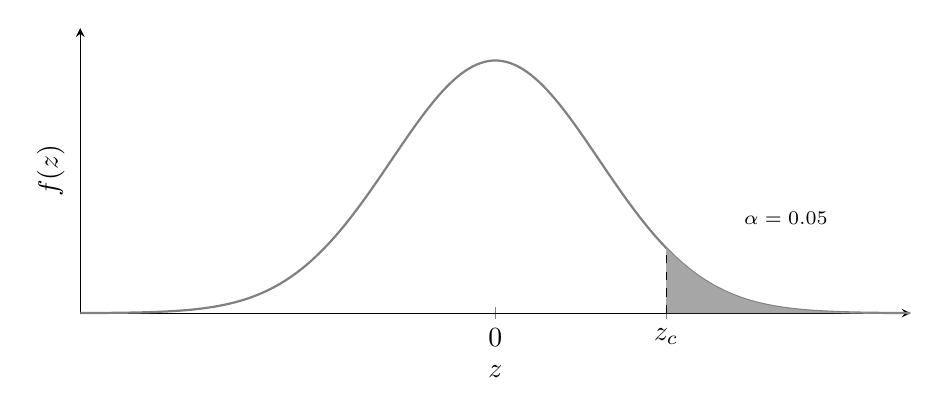
\begin{tikzpicture}
\begin{axis}[
width=\linewidth,
height=5.2cm,
xmin=-4,
xmax=4,
ymin=0,
ymax=0.45,
axis lines=left,
xlabel={$z$},
ylabel={$f(z)$},
xtick={0,1.645},
xticklabels={$0$,$z_c$},
ytick=\empty,
clip=false
]
\addplot[domain=-4:4,samples=200,thick,gray]{1/sqrt(2*pi)*exp(-x^2/2)};
\addplot[domain=1.645:4,draw=none,fill=black!35]{1/sqrt(2*pi)*exp(-x^2/2)}\closedcycle;
\draw[dashed](axis cs:1.645,0)--(axis cs:1.645,{1/sqrt(2*pi)*exp(-1.645^2/2)});
\node at (axis cs:2.8,0.15){\scriptsize $\alpha=0.05$};
\end{axis}
\end{tikzpicture}
\scriptsize
\end{column}
\end{columns}
\end{frame}

\begin{frame}{Module 1.2.3 : Estimation and Hypothesis Testing}
\scriptsize
\textbf{Example :} A roller bearing has a lifetime that is normally distributed with $\mu = 6000\text{hr}$ and $\sigma = 450\text{hr}$.  A sample of $n=9$ bearings manufactured using a new lubricant has an average lifetime of $\bar{x}=6400\text{hr}$. \\ \vspace{0.25cm}
\textbf{Question :} Has the new lubricant produced a statistically significant increase in mean lifetime?
\vspace{0.25cm}
\begin{columns}[T]
\begin{column}{0.58\textwidth}
\scriptsize
Assuming the \textit{population} standard deviation, $\sigma$, is known, the error in the mean is $\sigma/\sqrt{n}$, the z-score is 
\begin{equation}
z=\frac{\left|\mu-\bar{x}\right|}{\sigma/\sqrt{n}}
\end{equation}
Substituting the data, $P(Z<2.67)=0.996$, from the standard normal table. The probability of observing a result this
extreme by chance is therefore $0.004$. \\ \vspace{0.25cm}
\textbf{Result :} Only a $0.4\%$ chance exists that the increase in mean lifetime occurred randomly.
\end{column}
\begin{column}{0.42\textwidth}
\begin{tikzpicture}
\begin{axis}[
width=\linewidth,
height=5.2cm,
xmin=-4,
xmax=4,
ymin=0,
ymax=0.45,
axis lines=left,
xlabel={$z$},
ylabel={$f(z)$},
xtick={0,2.67},
xticklabels={$0$,$2.67$},
ytick=\empty,
clip=false
]
\addplot[domain=-4:4,samples=200,thick,gray]{1/sqrt(2*pi)*exp(-x^2/2)};
\addplot[domain=2.67:4,samples=100,draw=none,fill=black]{1/sqrt(2*pi)*exp(-x^2/2)}\closedcycle;
\draw[dashed](axis cs:2.67,0)--(axis cs:2.67,{1/sqrt(2*pi)*exp(-2.67^2/2)});
\node at (axis cs:3.2,0.05){\scriptsize $0.004$};
\end{axis}
\end{tikzpicture} \\
\scriptsize
Since $0.4\% < 5\%$, the result is significant.
\end{column}
\end{columns}
\end{frame}

\begin{frame}{Module 1.2.3 : Estimation and Hypothesis Testing}
\scriptsize
\textbf{Example :} Suppose two samples of bearings from the previous example are tested.  The first sample has a mean and standard deviation of 6000 hr and 450 hr ($n=60$). The second sample has a mean and standard deviation of 6400 hr and 380 hr ($n=9$). \\ \vspace{0.25cm}
\textbf{Question :} Is the difference in mean values still statistically significant?
\vspace{0.25cm}
\begin{columns}[T]
\begin{column}{0.58\textwidth}
\scriptsize
The standard deviation of the distribution of differences in the sample means is 
\begin{equation}
S_{\bar{x}_1 - \bar{x}_2} = \frac{\sigma_1}{\sqrt{n_1}}+\frac{\sigma_2}{\sqrt{n_2}}
\end{equation}
The z-score is the difference in sample means, divided by $S_{\bar{x}_1 - \bar{x}_2}$.  Substituting the data, $z = 400/185 - 2.16$, and $P(Z<2.16)=0.985$, from the standard normal table. The probability of observing a result this extreme by chance is therefore $0.015$. \\ \vspace{0.25cm}
\textbf{Result :} Only a $1.5\%$ chance exists that the increase in mean lifetime occurred randomly.
\end{column}
\begin{column}{0.42\textwidth}
\begin{tikzpicture}
\begin{axis}[
width=\linewidth,
height=5.2cm,
xmin=-4,
xmax=4,
ymin=0,
ymax=0.45,
axis lines=left,
xlabel={$z$},
ylabel={$f(z)$},
xtick={0,2.67},
xticklabels={$0$,$2.67$},
ytick=\empty,
clip=false
]
\addplot[domain=-4:4,samples=200,thick,gray]{1/sqrt(2*pi)*exp(-x^2/2)};
\addplot[domain=2.67:4,samples=100,draw=none,fill=black]{1/sqrt(2*pi)*exp(-x^2/2)}\closedcycle;
\draw[dashed](axis cs:2.67,0)--(axis cs:2.67,{1/sqrt(2*pi)*exp(-2.67^2/2)});
\node at (axis cs:3.2,0.05){\scriptsize $0.004$};
\end{axis}
\end{tikzpicture} \\
\scriptsize
Since $1.5\% < 5\%$, the result is significant.
\end{column}
\end{columns}
\end{frame}

\begin{frame}{Module 1.2.4 : Graphical and Tabular Methods}
\scriptsize
\textbf{Graphical techniques} are often useful to extract reliability parameters.  Consider the following histogram of failure times measured from $N$ units of the same electronic component.
\begin{columns}[T]
\begin{column}{0.45\textwidth}
\begin{table}
\begin{tabular}{c c c}
\hline
\textbf{Bin} & \textbf{Freq.} & \textbf{Exp. Freq.} \\
0-100 & 35 & 39.3 \\
100-200 & 26 & 23.8 \\
200-300 & 11 & 14.5 \\
300-400 & 12 & 8.8 \\
400-500 & 6 & 5.3 \\
500-600 & 3 & 3.2 \\
600-700 & 4 & 2.0 \\
700-800 & 2 & 1.2 \\
800-900 & 0 & 0.7 \\
900-1000 & 1 & 0.4 \\
\hline
\end{tabular}
\scriptsize
\caption{\scriptsize Histogram of failure times (columns 1 and 2), alongside predicted failure times (column 3). \label{tab:placeholder}}
\end{table}
\end{column}
\begin{column}{0.55\textwidth}
Assume the data follows the exponential distribution ($\lambda \approx 5\times 10^{-3}$ hr$^{-1}$.  The expected frequencies for events in each bin are:
\begin{equation}
\text{Exp. Freq.} = N\int_a^b \lambda e^{-\lambda t}dt
\end{equation}
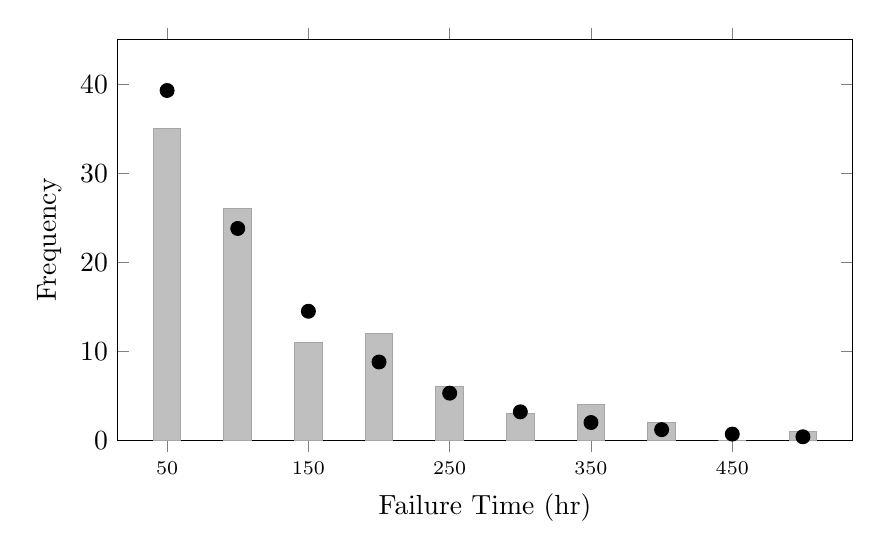
\begin{tikzpicture}
\begin{axis}[
    width=0.9\linewidth,
    height=0.55\linewidth,
    ybar,
    bar width=10pt,
    ymin=0,
    ymax=45,
    xlabel={Failure Time (hr)},
    ylabel={Frequency},
    xmin=0,
    xmax=1000,
    xtick={50,250,450,650,850},
    xticklabels={
        50,150,250,350,450,
        550,650,750,850,950
    },
    x tick label style={
        font=\scriptsize
    },
    ytick={0,10,20,30,40},
    legend style={
        at={(0.5,1.05)},
        anchor=south,
        legend columns=-1
    },
    enlarge x limits=0.02,
]
\addplot[ybar,fill=gray!50,draw=gray!70]
coordinates {
    (50,35)
    (150,26)
    (250,11)
    (350,12)
    (450,6)
    (550,3)
    (650,4)
    (750,2)
    (850,0)
    (950,1)
};
\addplot[only marks,black,mark=*,mark size=2.5pt]
coordinates {
    (50,39.3)
    (150,23.8)
    (250,14.5)
    (350,8.8)
    (450,5.3)
    (550,3.2)
    (650,2.0)
    (750,1.2)
    (850,0.7)
    (950,0.4)
};
\end{axis}
\end{tikzpicture} \\ \vspace{0.15cm}
\textbf{Circles :} expected frequencies.  \textbf{Bars :} observed frequencies.
\end{column}
\end{columns}
\end{frame}

\begin{frame}{Module 1.2.5 : Goodness-of-Fit Tests}
\scriptsize
\textbf{Goodness-of-fit tests} assess the agreement between predicted and observed distributions. \\ \vspace{0.25cm}
\begin{columns}[T]
\begin{column}{0.55\textwidth}
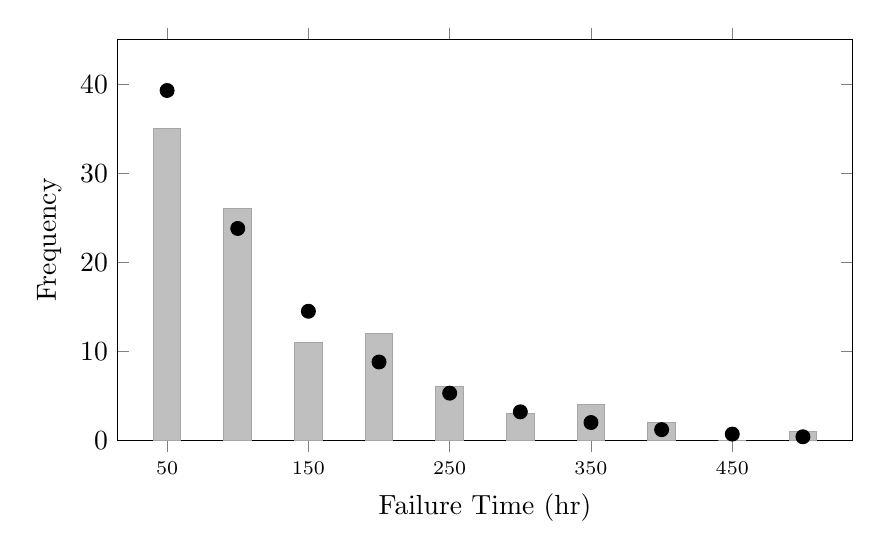
\begin{tikzpicture}
\begin{axis}[
    width=0.9\linewidth,
    height=0.55\linewidth,
    ybar,
    bar width=10pt,
    ymin=0,
    ymax=45,
    xlabel={Failure Time (hr)},
    ylabel={Frequency},
    xmin=0,
    xmax=1000,
    xtick={50,250,450,650,850},
    xticklabels={
        50,150,250,350,450,
        550,650,750,850,950
    },
    x tick label style={
        font=\scriptsize
    },
    ytick={0,10,20,30,40},
    legend style={
        at={(0.5,1.05)},
        anchor=south,
        legend columns=-1
    },
    enlarge x limits=0.02,
]
\addplot[ybar,fill=gray!50,draw=gray!70]
coordinates {
    (50,35)
    (150,26)
    (250,11)
    (350,12)
    (450,6)
    (550,3)
    (650,4)
    (750,2)
    (850,0)
    (950,1)
};
\addplot[only marks,black,mark=*,mark size=2.5pt]
coordinates {
    (50,39.3)
    (150,23.8)
    (250,14.5)
    (350,8.8)
    (450,5.3)
    (550,3.2)
    (650,2.0)
    (750,1.2)
    (850,0.7)
    (950,0.4)
};
\end{axis}
\end{tikzpicture} \\ \vspace{0.15cm}
Let $o_i$ represent the observations (gray bars), and $e_i$ represent the predictions (black circles).  The \textit{chi-square} test compares the following test statistic to the Chi-square PDF:
\begin{equation}
\chi^2 = \sum_{i=1}^N \frac{(o_i - e_i)^2}{e_i} \label{eq:chisq}
\end{equation}
\end{column}
\begin{column}{0.45\textwidth}
\textbf{Basic steps :}
\begin{itemize}
\item Choose distribution and confidence level (CL) $1-\alpha$
\item Let $N$ be the number of \textbf{bins}
\item Let $n$ be the number of distribution parameters
\item Calculate the sum in Eq. \ref{eq:chisq}
\item If the result is greater than $\chi^2_{1-\alpha}(N-n-1)$, reject the fit.
\item Else, accept the fit at CL $1-\alpha$.
\end{itemize}
\end{column}
\end{columns}
\end{frame}

\begin{frame}[fragile]{Module 1.2.5 : Goodness-of-Fit Tests}
\scriptsize
\begin{columns}[T]
\begin{column}{0.55\textwidth}
\begin{itemize}
\item Select exponential model, with $\lambda = 5\times 10^{-3}$ hr$^{-1}$.
\item $N = 10$, $n = 1$.
\item Calculate $\chi^2$ sum:
For the exponential failure model, $N-n-1 = 8$. The measured and expected frequencies give:
\begin{equation}
\chi^2 =\sum_{i=1}^{10}\frac{(o_i-e_i)^2}{e_i} = 6.92
\end{equation}
\item Compare to theoretical distribution:
\begin{align}
1-\alpha&=0.95 \\
\chi^2_{0.95}(8)&=15.51 \\
6.92 &< 15.51, \text{accept model}
\end{align}
\end{itemize}
\textbf{Microscoft Excel}, $\chi^2_{1-\alpha}(N-m-1)$:
\begin{verbatim}
=CHISQ.INV.RT(1-alpha,N-n-1)
\end{verbatim}
\end{column}
\begin{column}{0.45\textwidth}
\scriptsize
\textbf{Figure \ref{fig:chisq} :} Algorithms can also minimize the \textit{reduced chi-square}:
$\chi_r^2 = \frac{1}{N-n}\sum_{i=1}^{N}\frac{(f_i-f(x_i))^2}{\sigma_i^2}$. \\ \vspace{0.25cm}
Fitting the \textit{reduced chi-squared} to un-binned data is common in the physical sciences.
\begin{figure}
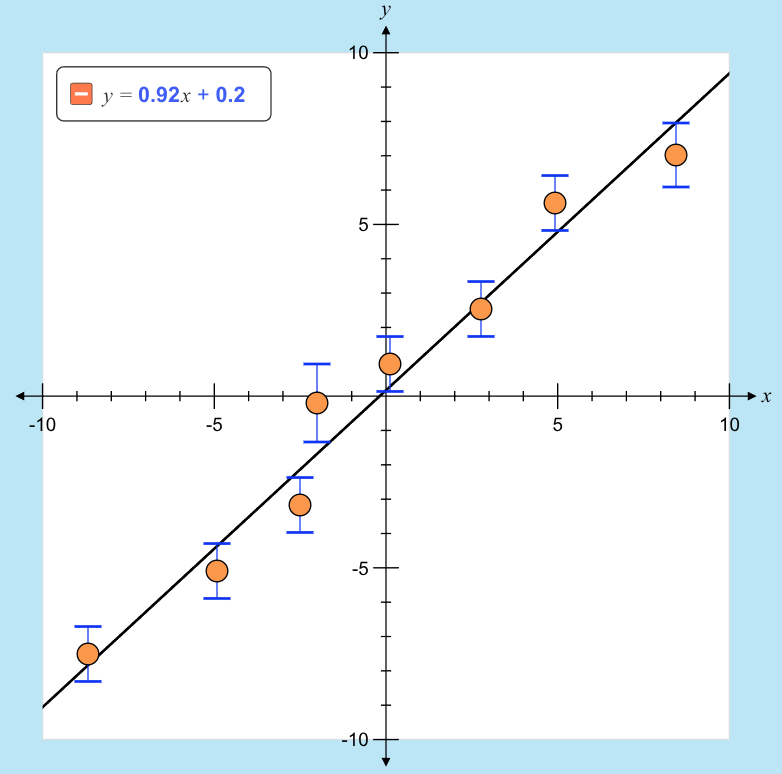
\includegraphics[width=0.9\linewidth]{chi-sq.png}
\caption{\label{fig:chisq}}
\end{figure}
\end{column}
\end{columns}
\end{frame}

\begin{frame}[fragile]{Module 1.2.5, 1.2.6 : Goodness-of-Fit Tests, Linear Regression}
\scriptsize
\textbf{Reduced chi-square} compares several candidate models while accounting
for the number of fitted parameters.  For example, consider the model table below.
\vspace{0.2cm}
\begin{columns}[T]
\begin{column}{0.56\textwidth}
\begin{tabular}{lccc}
\hline
\textbf{Model} & $\chi^2$ & $\chi_r^2$ & Result\\
\hline
Exponential & 16.8 & 2.40 & Poor fit\\
Lognormal   & 10.8 & 1.54 & Acceptable\\
Weibull ($\beta=1.35$) & 7.1 & 1.01 & Best fit\\
\hline
\end{tabular} \\ \vspace{0.25cm}
For all three models, the degrees of freedom (dof) are $N-n-1=7$.  The reduced chi-square is computed as
\begin{equation}
\chi_r^2=\frac{\chi^2}{dof}.
\end{equation}
For the Weibull model, $\chi_r^2 = 7.1/7 = 1.01$. The interpretation of $\chi_r^2$ is as follows:
\begin{itemize}
\item $\chi_r^2\gg1$: model poorly explains the data.
\item $\chi_r^2\approx1$: model agrees with observations.
\item $\chi_r^2\ll1$: over-fitting the data.
\end{itemize}
\end{column}
\begin{column}{0.44\textwidth}
The Weibull model has the smallest $\chi_r^2$, so $\beta=1.35$ is selected. \\ \vspace{0.25cm}
Note: when tuning $\beta$ to minimize $\chi_r^2$
\begin{itemize}
    \item $\beta > 1$ indicates failure rate is increasing with time.
    \item $\beta < 1$ indicates failure rate is decreasing with time.
\end{itemize}
\textbf{Linearized} data $\Rightarrow$ regression techniques: \\ \vspace{0.25cm}
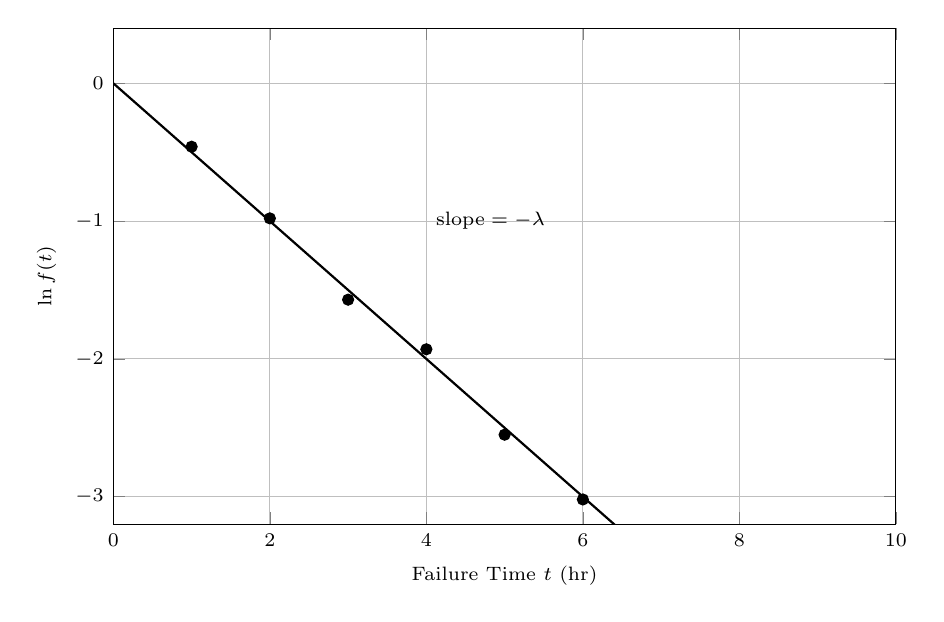
\begin{tikzpicture}
\begin{axis}[
    width=0.95\linewidth,
    height=0.65\linewidth,
    xlabel={Failure Time $t$ (hr)},
    ylabel={$\ln f(t)$},
    xmin=0,xmax=10,
    ymin=-3.2,ymax=0.4,
    xtick={0,2,4,6,8,10},
    ytick={-3,-2,-1,0},
    grid=major,
    tick label style={font=\scriptsize},
    label style={font=\scriptsize},
]

% Best-fit line
\addplot[
    black,
    thick,
    domain=0:10,
    samples=2
]
{-0.5*x};

% Sample data
\addplot[
    only marks,
    mark=*,
    mark size=2pt,
    black
]
coordinates{
    (1,-0.46)
    (2,-0.98)
    (3,-1.57)
    (4,-1.93)
    (5,-2.55)
    (6,-3.02)
};

% Slope annotation
\node[anchor=west,font=\scriptsize]
at (axis cs:4,-1.0)
{$\text{slope}=-\lambda$};

\end{axis}
\end{tikzpicture}
\end{column}
\end{columns}
\end{frame}

\end{document}